% Options for packages loaded elsewhere
\PassOptionsToPackage{unicode}{hyperref}
\PassOptionsToPackage{hyphens}{url}
%
\documentclass[
]{book}
\usepackage{amsmath,amssymb}
\usepackage{iftex}
\ifPDFTeX
  \usepackage[T1]{fontenc}
  \usepackage[utf8]{inputenc}
  \usepackage{textcomp} % provide euro and other symbols
\else % if luatex or xetex
  \usepackage{unicode-math} % this also loads fontspec
  \defaultfontfeatures{Scale=MatchLowercase}
  \defaultfontfeatures[\rmfamily]{Ligatures=TeX,Scale=1}
\fi
\usepackage{lmodern}
\ifPDFTeX\else
  % xetex/luatex font selection
\fi
% Use upquote if available, for straight quotes in verbatim environments
\IfFileExists{upquote.sty}{\usepackage{upquote}}{}
\IfFileExists{microtype.sty}{% use microtype if available
  \usepackage[]{microtype}
  \UseMicrotypeSet[protrusion]{basicmath} % disable protrusion for tt fonts
}{}
\makeatletter
\@ifundefined{KOMAClassName}{% if non-KOMA class
  \IfFileExists{parskip.sty}{%
    \usepackage{parskip}
  }{% else
    \setlength{\parindent}{0pt}
    \setlength{\parskip}{6pt plus 2pt minus 1pt}}
}{% if KOMA class
  \KOMAoptions{parskip=half}}
\makeatother
\usepackage{xcolor}
\usepackage{color}
\usepackage{fancyvrb}
\newcommand{\VerbBar}{|}
\newcommand{\VERB}{\Verb[commandchars=\\\{\}]}
\DefineVerbatimEnvironment{Highlighting}{Verbatim}{commandchars=\\\{\}}
% Add ',fontsize=\small' for more characters per line
\usepackage{framed}
\definecolor{shadecolor}{RGB}{248,248,248}
\newenvironment{Shaded}{\begin{snugshade}}{\end{snugshade}}
\newcommand{\AlertTok}[1]{\textcolor[rgb]{0.94,0.16,0.16}{#1}}
\newcommand{\AnnotationTok}[1]{\textcolor[rgb]{0.56,0.35,0.01}{\textbf{\textit{#1}}}}
\newcommand{\AttributeTok}[1]{\textcolor[rgb]{0.13,0.29,0.53}{#1}}
\newcommand{\BaseNTok}[1]{\textcolor[rgb]{0.00,0.00,0.81}{#1}}
\newcommand{\BuiltInTok}[1]{#1}
\newcommand{\CharTok}[1]{\textcolor[rgb]{0.31,0.60,0.02}{#1}}
\newcommand{\CommentTok}[1]{\textcolor[rgb]{0.56,0.35,0.01}{\textit{#1}}}
\newcommand{\CommentVarTok}[1]{\textcolor[rgb]{0.56,0.35,0.01}{\textbf{\textit{#1}}}}
\newcommand{\ConstantTok}[1]{\textcolor[rgb]{0.56,0.35,0.01}{#1}}
\newcommand{\ControlFlowTok}[1]{\textcolor[rgb]{0.13,0.29,0.53}{\textbf{#1}}}
\newcommand{\DataTypeTok}[1]{\textcolor[rgb]{0.13,0.29,0.53}{#1}}
\newcommand{\DecValTok}[1]{\textcolor[rgb]{0.00,0.00,0.81}{#1}}
\newcommand{\DocumentationTok}[1]{\textcolor[rgb]{0.56,0.35,0.01}{\textbf{\textit{#1}}}}
\newcommand{\ErrorTok}[1]{\textcolor[rgb]{0.64,0.00,0.00}{\textbf{#1}}}
\newcommand{\ExtensionTok}[1]{#1}
\newcommand{\FloatTok}[1]{\textcolor[rgb]{0.00,0.00,0.81}{#1}}
\newcommand{\FunctionTok}[1]{\textcolor[rgb]{0.13,0.29,0.53}{\textbf{#1}}}
\newcommand{\ImportTok}[1]{#1}
\newcommand{\InformationTok}[1]{\textcolor[rgb]{0.56,0.35,0.01}{\textbf{\textit{#1}}}}
\newcommand{\KeywordTok}[1]{\textcolor[rgb]{0.13,0.29,0.53}{\textbf{#1}}}
\newcommand{\NormalTok}[1]{#1}
\newcommand{\OperatorTok}[1]{\textcolor[rgb]{0.81,0.36,0.00}{\textbf{#1}}}
\newcommand{\OtherTok}[1]{\textcolor[rgb]{0.56,0.35,0.01}{#1}}
\newcommand{\PreprocessorTok}[1]{\textcolor[rgb]{0.56,0.35,0.01}{\textit{#1}}}
\newcommand{\RegionMarkerTok}[1]{#1}
\newcommand{\SpecialCharTok}[1]{\textcolor[rgb]{0.81,0.36,0.00}{\textbf{#1}}}
\newcommand{\SpecialStringTok}[1]{\textcolor[rgb]{0.31,0.60,0.02}{#1}}
\newcommand{\StringTok}[1]{\textcolor[rgb]{0.31,0.60,0.02}{#1}}
\newcommand{\VariableTok}[1]{\textcolor[rgb]{0.00,0.00,0.00}{#1}}
\newcommand{\VerbatimStringTok}[1]{\textcolor[rgb]{0.31,0.60,0.02}{#1}}
\newcommand{\WarningTok}[1]{\textcolor[rgb]{0.56,0.35,0.01}{\textbf{\textit{#1}}}}
\usepackage{longtable,booktabs,array}
\usepackage{calc} % for calculating minipage widths
% Correct order of tables after \paragraph or \subparagraph
\usepackage{etoolbox}
\makeatletter
\patchcmd\longtable{\par}{\if@noskipsec\mbox{}\fi\par}{}{}
\makeatother
% Allow footnotes in longtable head/foot
\IfFileExists{footnotehyper.sty}{\usepackage{footnotehyper}}{\usepackage{footnote}}
\makesavenoteenv{longtable}
\usepackage{graphicx}
\makeatletter
\def\maxwidth{\ifdim\Gin@nat@width>\linewidth\linewidth\else\Gin@nat@width\fi}
\def\maxheight{\ifdim\Gin@nat@height>\textheight\textheight\else\Gin@nat@height\fi}
\makeatother
% Scale images if necessary, so that they will not overflow the page
% margins by default, and it is still possible to overwrite the defaults
% using explicit options in \includegraphics[width, height, ...]{}
\setkeys{Gin}{width=\maxwidth,height=\maxheight,keepaspectratio}
% Set default figure placement to htbp
\makeatletter
\def\fps@figure{htbp}
\makeatother
\setlength{\emergencystretch}{3em} % prevent overfull lines
\providecommand{\tightlist}{%
  \setlength{\itemsep}{0pt}\setlength{\parskip}{0pt}}
\setcounter{secnumdepth}{5}
\usepackage{booktabs}
\ifLuaTeX
  \usepackage{selnolig}  % disable illegal ligatures
\fi
\usepackage[]{natbib}
\bibliographystyle{plainnat}
\IfFileExists{bookmark.sty}{\usepackage{bookmark}}{\usepackage{hyperref}}
\IfFileExists{xurl.sty}{\usepackage{xurl}}{} % add URL line breaks if available
\urlstyle{same}
\hypersetup{
  pdftitle={Descriptive statistics},
  pdfauthor={Sara Souther},
  hidelinks,
  pdfcreator={LaTeX via pandoc}}

\title{Descriptive statistics}
\author{Sara Souther}
\date{2024-09-19}

\begin{document}
\maketitle

{
\setcounter{tocdepth}{1}
\tableofcontents
}
\hypertarget{ecological-data-analysis-in-env-226-laboratory}{%
\chapter{Ecological data analysis in ENV 226 laboratory}\label{ecological-data-analysis-in-env-226-laboratory}}

This course surveys the central concepts in ecology: evolution, population dynamics, community interactions, biogeochemical cycling, and limiting factors, as well as how those factors are measured, quantified, and interact with drivers of global environmental change. This course is required for the B.S. in Environmental Sciences degree program, and also the B.S. in Environmental and Sustainability Studies degree. This course acquaints students with foundational concepts and theories in ecology and provides a broad basis for more advanced courses in subdisciplines and applications of ecology.

A critical part of ecological research is developing practical and analytic skills. Most ecologists and data scientists use R statistical software. Learning how to manage, manipulate and analyze data in R will serve your undergraduate career and beyond! In ENV 226 lab, we will ease you into using R for all your data needs!

\hypertarget{how-to-use-this-resource}{%
\section{How to use this resource}\label{how-to-use-this-resource}}

Each chapter in this online book corresponds to a lesson that will help you in lab. When starting a new chapter, create a new R script with a name that allows you to easily connect the content in the R script to the chapter. Then, copy and paste sections of code in the chapter into your R script to practice!

\begin{Shaded}
\begin{Highlighting}[]
\NormalTok{knitr}\SpecialCharTok{::}\NormalTok{opts\_chunk}\SpecialCharTok{$}\FunctionTok{set}\NormalTok{(}\AttributeTok{warning =} \ConstantTok{FALSE}\NormalTok{, }\AttributeTok{message =} \ConstantTok{FALSE}\NormalTok{)}
\end{Highlighting}
\end{Shaded}

\hypertarget{welcome-to-r}{%
\chapter{Welcome to R!}\label{welcome-to-r}}

R is an open source statistical software package commonly used by researchers and other folks, who crave a free way to manipulate, analyze, and visualize date. R uses it's own programming language, which is similar to S+ (the paid precursor to R). R employs an object-oriented programming (OOP) paradigm, specifically a type of OOP known as ``class-based object-oriented programming,'' to manage and manipulate data. In R, objects are fundamental entities, and you work with data and functions through objects. Let's walk through the basics of installing and using R!

\hypertarget{r-and-r-studio-installation}{%
\section{R and R studio installation}\label{r-and-r-studio-installation}}

You will first want to download R statistical software and R studio, which is a powerful program that interfaces with R to make your coding experience more organized and enjoyable. Notice that you need to select a version of R depending on your operating system.

\hypertarget{download-the-r-statistical-software-from-the-official-r-project-website.}{%
\section{Download the R statistical software from the official R Project website.}\label{download-the-r-statistical-software-from-the-official-r-project-website.}}

Open your web browser and go to the official R Project website at \url{https://www.r-project.org/}.

Choose a CRAN Mirror: On the R Project website's main page, you'll see a section that says ``Download and Install R.'' Click on the link that says ``CRAN (Comprehensive R Archive Network).'' This will take you to the CRAN website.

\begin{enumerate}
\def\labelenumi{\arabic{enumi}.}
\item
  Select Your Mirror: On the CRAN website, you'll find a list of mirrors (servers) from which you can download R. Choose a mirror that is geographically close to your location, as this will generally provide faster download speeds. Click on the mirror's link.
\item
  Download R for Your Operating System: On the mirror's page, you'll see options to download R for various operating systems (e.g., Windows, macOS, Linux). Click on the appropriate link for your operating system.
\item
  Choose the Latest Version: You'll typically see multiple versions of R available for download. It's recommended to choose the latest stable version unless you have a specific reason to use an older version.
\item
  Download and Install: After clicking on the download link, the installation file for R will begin downloading. Once the download is complete, run the installer and follow the installation instructions for your operating system.
\item
  Start Using R: After the installation is complete, you can launch R from your computer. Depending on your operating system, you may also have an option to install RStudio, a popular integrated development environment (IDE) for R, to enhance your R programming experience.
\end{enumerate}

\hypertarget{download-r-studio}{%
\section{Download R studio}\label{download-r-studio}}

Now download R studio!

\begin{enumerate}
\def\labelenumi{\arabic{enumi}.}
\item
  Visit the RStudio Website: Open your web browser and go to the official RStudio website at \url{https://www.rstudio.com/}.
\item
  Download RStudio: On the RStudio website's main page, click on the ``Products'' menu at the top, and then select ``RStudio'' from the dropdown menu.
\item
  Choose the RStudio Edition: RStudio offers different editions, including RStudio Desktop (for use on your local machine), RStudio Server (for remote access), and RStudio Workbench (formerly known as RStudio Server Pro, designed for collaboration and sharing in enterprise environments). You will want to choose the free version, RStudio Desktop.
\item
  Download the Installer: After selecting the edition, you'll be directed to a page with download options. Click on the download link for your operating system (e.g., Windows, macOS, Linux).
\item
  Download and Install: The installation file for RStudio will begin downloading. Once the download is complete, run the installer and follow the installation instructions for your operating system.
\end{enumerate}

Start Using RStudio: After the installation is complete, you can launch RStudio from your computer. You'll have access to a powerful IDE that provides a user-friendly interface for working with R, including code editing, interactive R console, data visualization, and more. RStudio greatly enhances your R programming and data analysis experience, and it's widely used by R users for its features and capabilities.

\hypertarget{set-up-r-studio}{%
\section{Set up R studio}\label{set-up-r-studio}}

Alright, now that you've downloaded R and R studio, open R studio. You can customize the panes that you are visualizing in R.

In RStudio, the four panels or panes are commonly referred to as:

\textbf{Source Pane}: This is where you can write, edit, and save your R scripts and code files. It is typically used for script development and editing. You can open and create new R script files in this pane.

\textbf{Console Pane}: The console is where you interact with R directly. You can execute R commands and see their output here. It's an interactive environment where you can test and run R code line by line or in batches.

\textbf{Environment Pane}: The environment pane displays information about the objects, data frames, variables, and functions currently loaded in your R session. You can also use this pane to view data frames in a spreadsheet-like format and manage your workspace.

\textbf{Files/Plots/Packages/Help Pane}: This pane has multiple tabs and serves various purposes:
\emph{Files}: It shows the file system of your project, allowing you to navigate and manage files and directories.
\emph{Plots}: When you create plots in R, they will appear in this tab. You can interact with and export the plots from here.
\emph{Packages}: This tab displays information about installed packages, and you can use it to install, update, or load packages.
\emph{Help}: When you need documentation or help for R functions or packages, you can use the Help tab to search for and view documentation.

Typically, I select a structure in which I have my \textbf{Source pane} in the upper left, my \textbf{Console Pane} in the lower left position, my \textbf{Environment Pane} in the upper right corner, and the \textbf{Files/Plots/Packages/Help Pane} in the lower right position. You can select any position that you'd like, but if we create the same work environment, it will be easy for me to direct you when we are trouble-shooting code. To adjust the panels positions, use the pane layout function. Here's what that looks at for a Mac, but typically this arrangement is the default positioning for panels in R studio, so you likely won't have to adjust positioning!

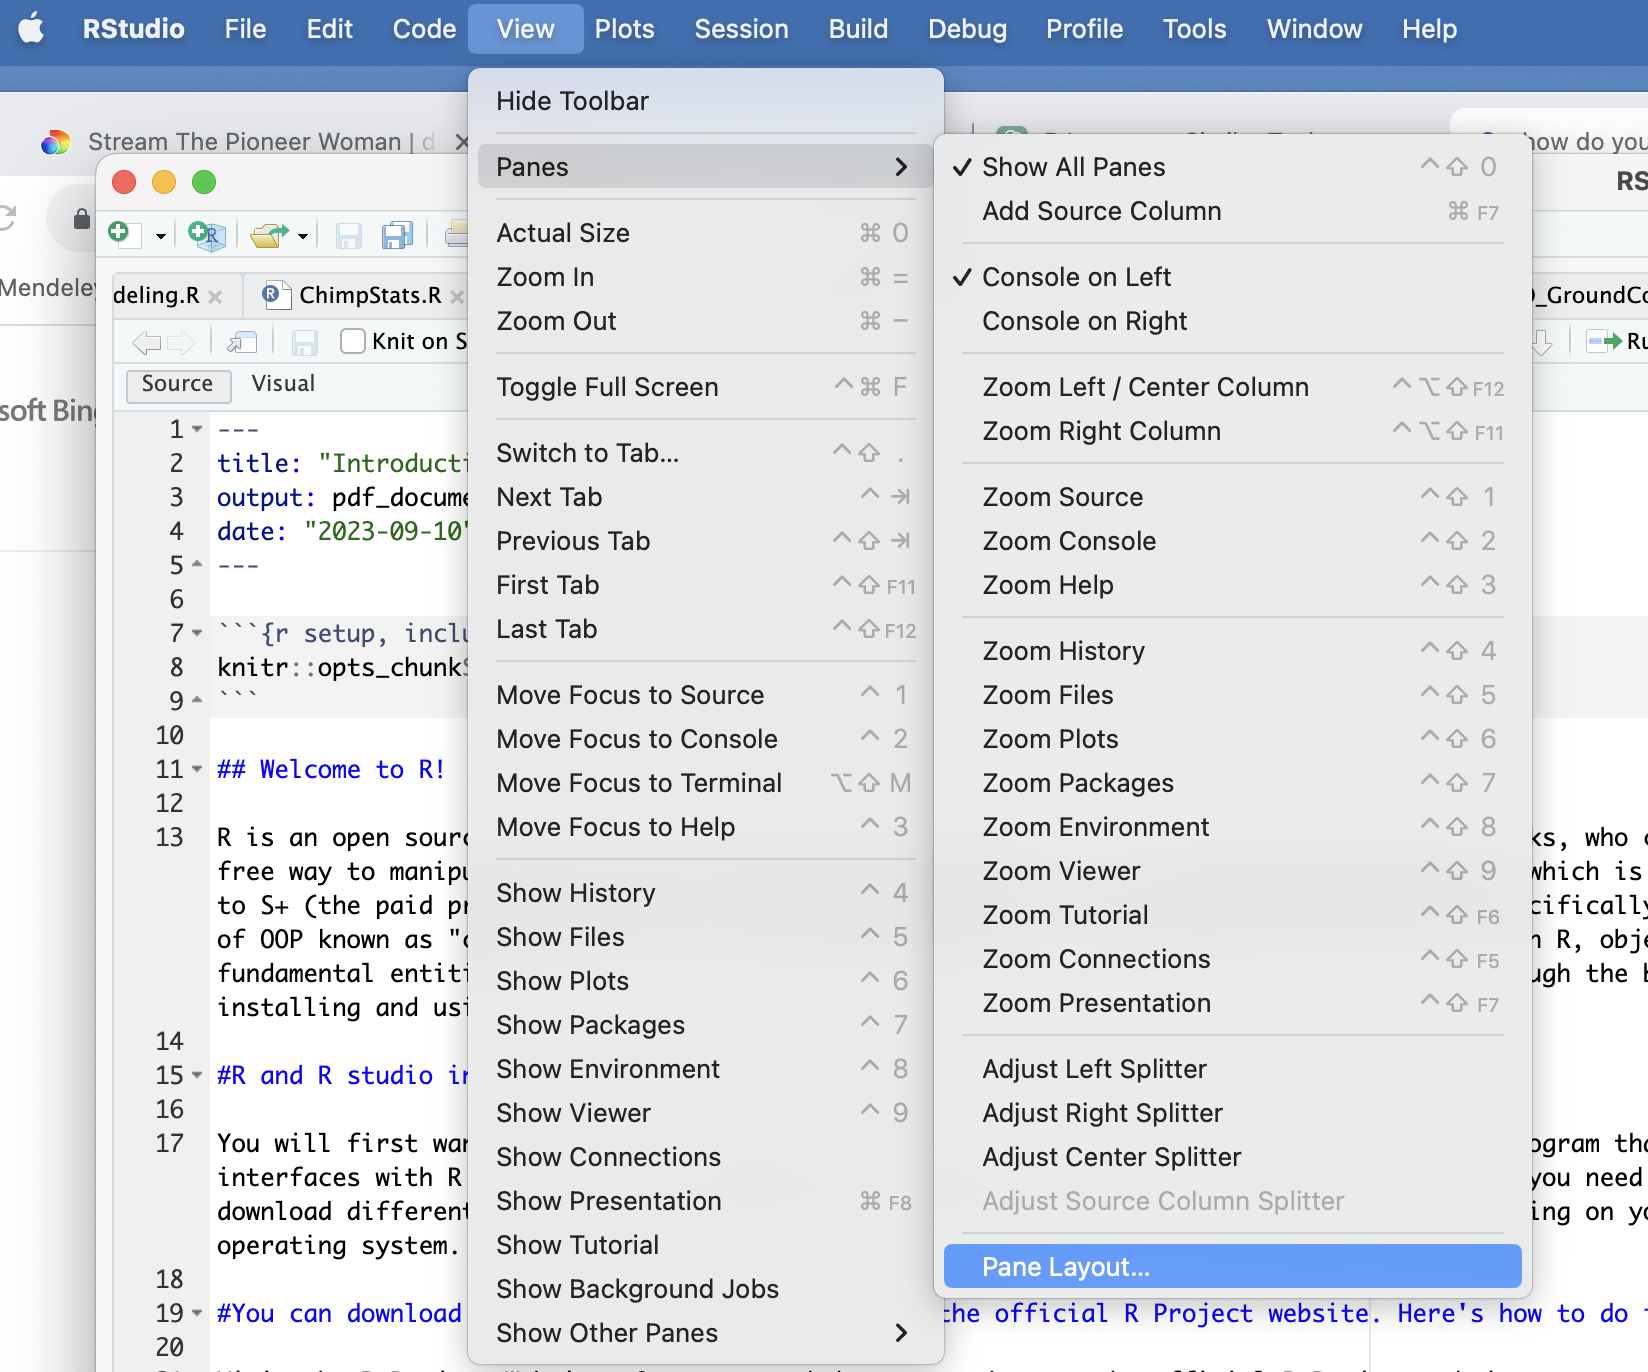
\includegraphics{images/01-intro/PaneLayout.png}

\hypertarget{good-housekeeping}{%
\section{Good housekeeping}\label{good-housekeeping}}

When you are coding in R, you will want to save your R or R markdown scripts and any other data files (e.g., .csv or spatial files) that you are analyzing in a common file. With good housekeeping, you will be able to seamlessly rerun your analyses at in point in time, allowing you to pick back up on projects that may have been dormant!

The first step in good R housekeeping is to set a \textbf{working directory}. A working directory tells R where to look for and save files. As an example, let's say I am planning to save everything associated with this tutorial to a file called Class1\_IntroToR. To do this, create a new folder on your desktop called `R is great'. You can change your working directory using the R studio interface by selecting a working directory at the top of the console panel in the ``Files'' tab. If you want to change your working directory to a different location, click on the ``\ldots{}'' (ellipsis) button in RStudio's ``Files'' tab. This will allow you to browse your file system and select a new directory as your working directory. That said, you will be \emph{far} better served by including code in your R script that directs R to your working directory. I prefer to set it within the code in order to allow you to instantaneously be able to pick up work where you left off rather than searching through files and trying to remember how you set up the code. You can view your working directory by running a simple bit of code (run code below).

\begin{Shaded}
\begin{Highlighting}[]
\FunctionTok{getwd}\NormalTok{() }\CommentTok{\#display file path to R studio }
\end{Highlighting}
\end{Shaded}

\begin{verbatim}
## [1] "/Users/sks379/Desktop/ENV226LabRManual"
\end{verbatim}

When you run, getwd() you will see where R is looking for files. Now, let's tell R where we want it to access files from! First, you will need to identify your file path. To find the file path to the Class1\_IntroToR on a mac, double click on the file and should see several option, including `Get info' (check out picture below).

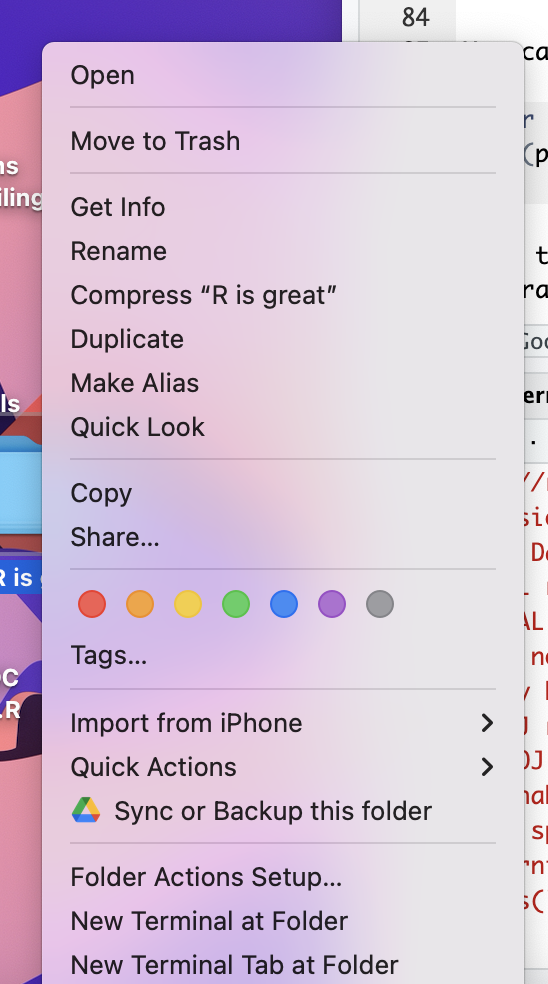
\includegraphics{images/01-intro/workingdirectorymac.png}
Then, select `Get info'. Then, highlight the information after `where' and copy it as a pathname (see picture).

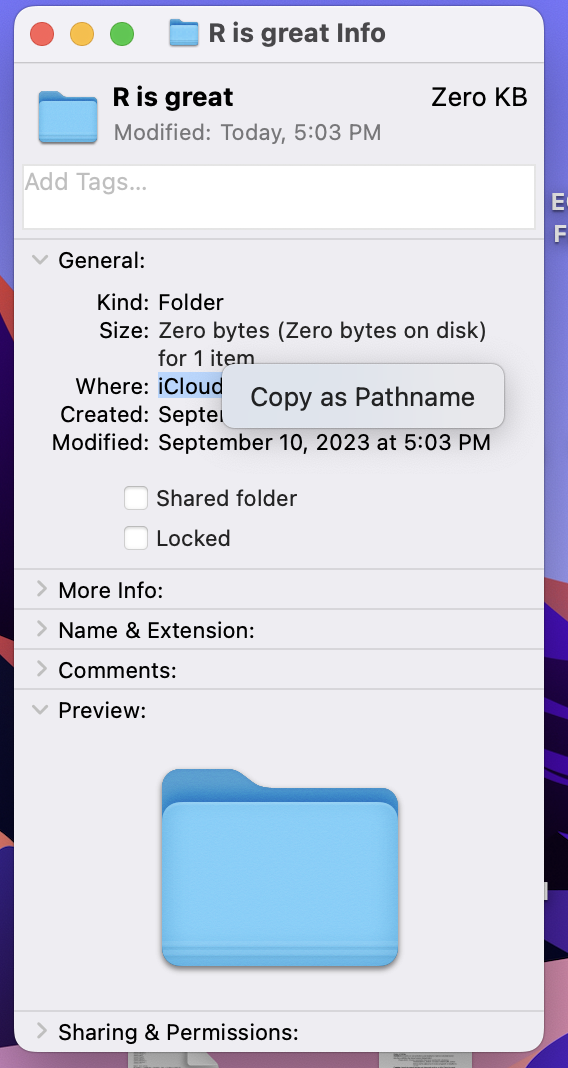
\includegraphics{images/01-intro/copyingpathnamemac.png}

For PCs, start by opening your File Explorer:
Press the Windows key + E on your keyboard.
Alternatively, you can click the ``File Explorer'' or ``This PC'' icon on your taskbar or Start menu.
Navigate to the Folder: Use the File Explorer to navigate to the folder where the file is located. You can click on folders to open them and view their contents.

\begin{enumerate}
\def\labelenumi{\arabic{enumi}.}
\item
  Find the File: Locate the file you are interested in within the folder.
\item
  View the File Path: Once you've found the file, you can see its full file path in the address bar at the top of the File Explorer window. The file path will be displayed as a sequence of folder and file names separated by backslashes. You can click in the address bar and copy the file path to the clipboard by pressing Ctrl + C after selecting it.
\item
  Once you have copied your file path, paste that path name into the following code and set your working directory: setwd(``/Users/sks379/Desktop/R is great/'')
\end{enumerate}

Now R studio is directed to upload and save work to this folder.

\hypertarget{annotating-your-code}{%
\section{Annotating your code}\label{annotating-your-code}}

Notice anything about the code in the section you just ran? You can use the hast tag symbol to tell R not to run a section of code. Whenever I am generating code, I try to add lots of notes to myself, so that that future me knows what code I created and why. Annotating your code is just good practice for coding! Alternatively, you can create R markdown files (what this tutorial has been created in), but R markdown, while generating pretty PDFs and websites, adds an extra layer of complexity that you generally don't want or need while coding, so I typically recommend creating an R script and annotating your that file! One thing that you might want to include in your code description is the version of R that you are using (you may need to load older versions of R if your scripts stop working due to updates to the program). To check the version of R that you are using, paste this in the command line: R.version.string

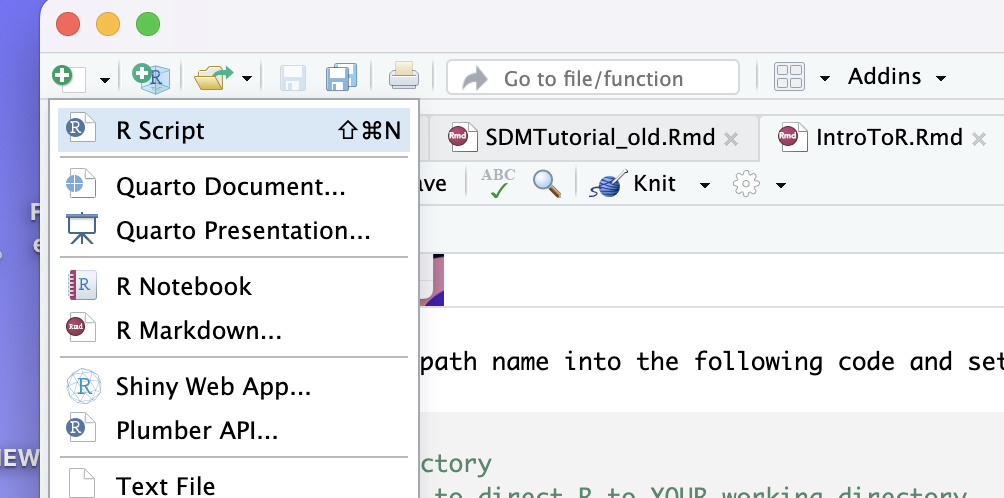
\includegraphics{images/01-intro/createrscript.png}

\hypertarget{libraries}{%
\section{Libraries}\label{libraries}}

Base R, the fundamental, built-in set of functions, data structures, and libraries that come with the R programming language without the need for additional packages or extensions, including basic math functions, statistical analyses and visualization tools. However, one amazingly cool think about R is that folks are out there creating `libraries', or a collection of R functions, data sets, and documentation bundled together into a single package, to do specialized analyses. For most tasks in R, you will need to install and load libraries. There are two methods to install libraries. Let's start by installing an important library (or package) for data manipulation, called `tidyverse' (actually several packages - hence why the name references a universe). To do this, run this code: install.packages(``tidyverse'').

The weird thing about including install packages code is that you don't want to re-install packages every time that you use R (in fact, it caused my R markdown code to freak out, which is why I've included the install function in the text). You will need to load packages, but you update R and R studio, you won't need to install packages after you have done it once. You can either then install the packages and delete the install code OR you can install through the R studio interface by going to packages, selecting install and searching for and installing the packages that you are interested in. When prompted, be sure to install dependencies - this will make sure that you have any pieces of code that the library that you are installing needs to operate.

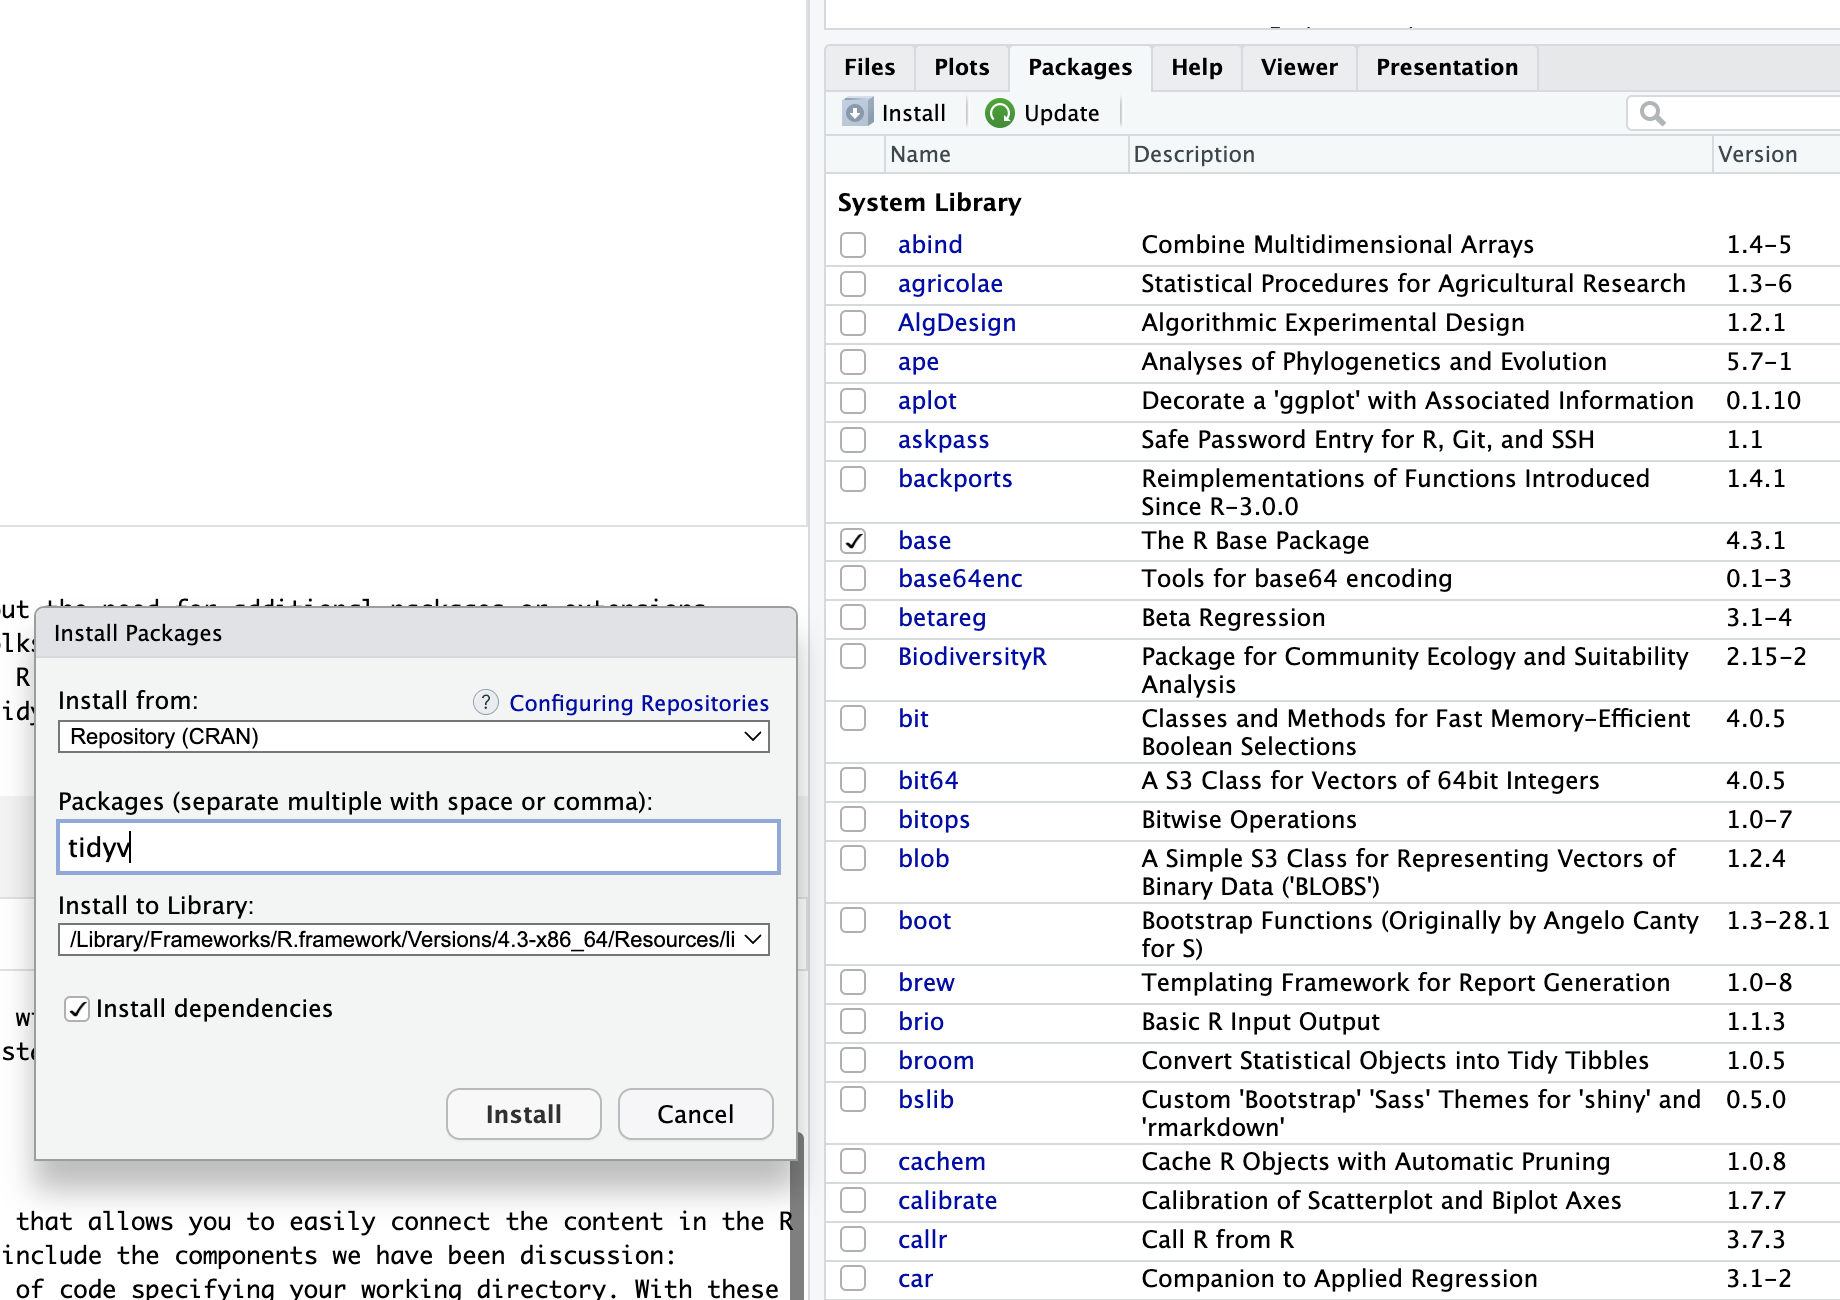
\includegraphics{images/01-intro/installlibraries.png}

Excellent! You have installed a library! Now, we need to load it. AND you will need to load R packages everytime that you use R. Any functions associated with your package won't work, unless the package is loaded, so I suggest keeping the load library code in your R script. The code is simple (see below).

\begin{Shaded}
\begin{Highlighting}[]
\FunctionTok{library}\NormalTok{(tidyverse)}
\end{Highlighting}
\end{Shaded}

Wonderful, you now have the essential knowledge base that you need to start working efficiently and effectively in R!

\hypertarget{organizing-your-code}{%
\section{Organizing your code}\label{organizing-your-code}}

A well-written R script will include the components we have been discussion: Annotated notes on what the script is doing and potentially even the version of R, loading commands for your libraries, and a line of code specifying your working directory. With these elements in place, you are ready to code your heart out!

Here is a glimpse at what your R scripts should look like.
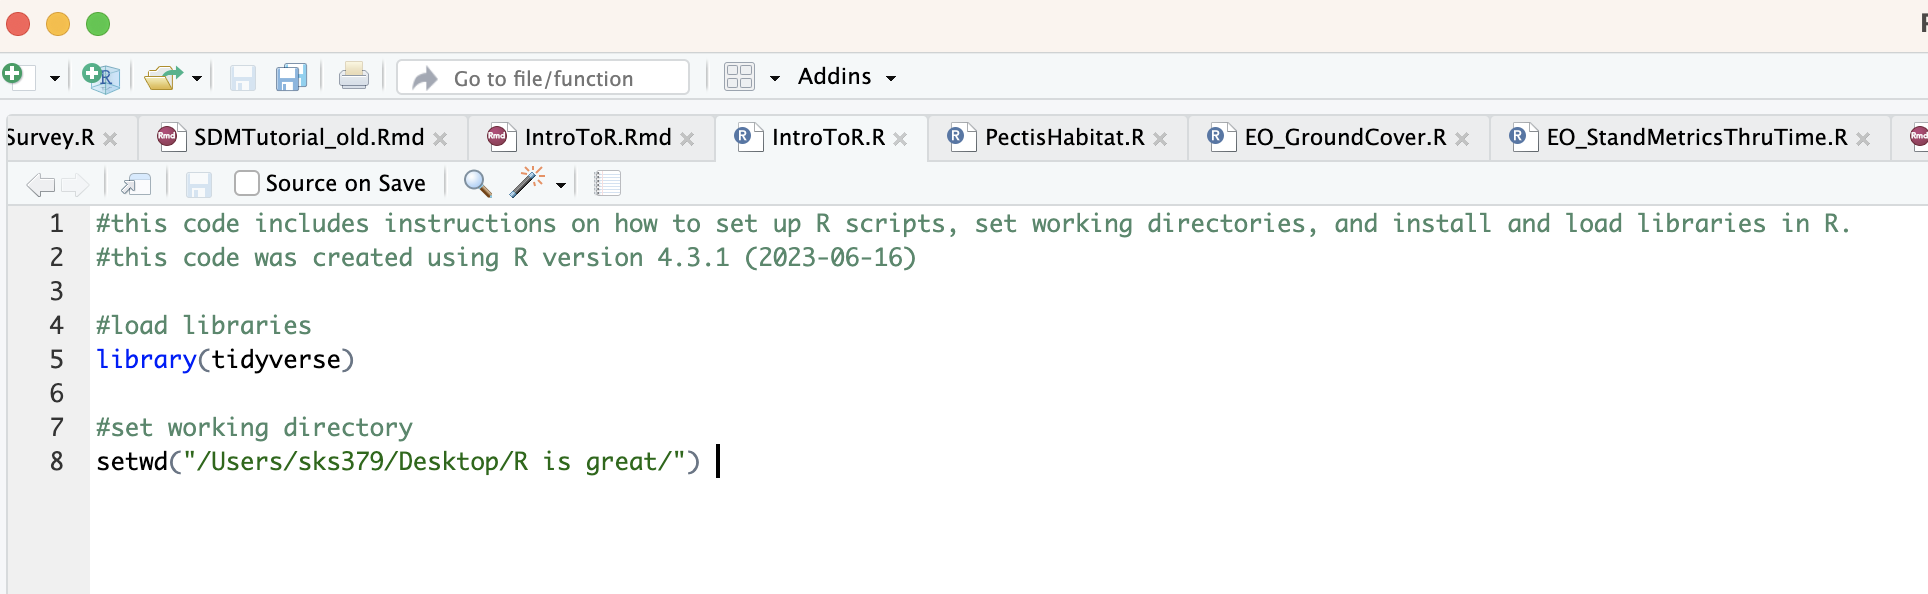
\includegraphics{images/01-intro/RScriptSetUp.png}

And with that, welcome to the wonderful world of coding in R!

\hypertarget{descriptive-statistics}{%
\chapter{Descriptive statistics}\label{descriptive-statistics}}

\hypertarget{what-can-statistics-tell-us}{%
\section{What can statistics tell us?}\label{what-can-statistics-tell-us}}

Welcome to our statistical exploration of the natural world! I want you to have an intuitive understanding of what we do when we conduct statistical analysis, understand how to select the appropriate statistical analysis and the assumptions of that analysis, and make a connection between running an analysis in a statistical software package and the statisticese of those unique individuals that we call statisticians. I think this will give you the confidence to tackle any analytical situation!

First off, we are \textbf{not} statisticians - whew! We are training to be ecologists. This means that we do not need to understand theoretical mathematical frameworks. We need to APPLY statistics appropriately. There will be limits to our mathematical understanding of statistics, and this is OKAY! Think of all of the knowledge about the natural world and conducting field work that we possess that statisticians don't!

Almost all statistical analysis boils down to answering 1 of 2 questions:
\emph{Do these groups differ?
}Is there a relationship between these variables?

These seem like relatively simple questions to answer, perhaps just by looking at our data, so \textbf{Why do we need statistics?}

The short answer is: \textbf{error} and \textbf{sampling}! Whenever we collect data, we introduce \textbf{error}; our instruments are imprecise and do not capture an exact measure of whatever you are measuring (e.g., height, weight), and humans make mistakes during measurement collection. Secondly, we are \textbf{always} measuring a sub-sample of the true population (\emph{true population} meaning all representatives of whatever you are trying to measure; this can be grass, marbles, or the tibia of humans). Not only is in intractable in most cases to measure all individuals of whatever you are interested in, even when it is possible to attempt to measure \textbf{all} individuals (like in the case of rare plant work), statistics acknowledges that it is \textbf{still} unlikely that we are able to completely measure all individuals in your focal population, since individuals may be dormant or challenging to locate. If we could measure all individuals of our population of interest with perfect accurately, we could calculate population \textbf{parameters}, or quantities describing populations like averages and variation, rather than estimating these metrics, and just compare them. In this way, statistics is inherently practical, and asks: What can we say about whatever we are looking at, given our numerous flaws?

\hypertarget{sampling-populations}{%
\section{Sampling populations}\label{sampling-populations}}

After a few classes, we will explore sampling methodology in greater depth in order to design appropriate experiments that test a statistical \textbf{hypothesis}. Let's quickly talk about sampling now so that we have a shared understanding and vocabulary to build on - after all, statistics really centers around estimating characteristics of a true population from a sample. The \textbf{really, truly} amazing thing is that by properly applying statistics, we can learn practically anything about almost any population using samples!

In statistics, a \textbf{population} refers to the all units of the thing that you are interested (i.e., all suriname frogs, all grains of sand, all aspen leaves from a genotype found in southern Arizona). \textbf{Note}: Population in statistics differs from the term population in population ecology, where a population refers to a group of individuals in a particular area that interbreed.

A \textbf{sample} is a subset of the population that we measure to infer something about the population. Statistical analyses depend on a random sample or must account for non-randomness within the sample. Just imagine, for instance, that you were interested in whether coat color in cats differed between house cats and feral cats. To select the house cat sample, you randomly select house numbers, visit the house and record coat color, thus collecting a random sample. However, to survey feral cats, you go to several cat colonies at night and record the first cat that you see, which are always white or tan. The sample of feral cats introduces bias, and causes you to overestimate the number of light colored feral cats, and underestimate dark feral cats.

We can conduct statistical analysis until the cats come home (ha!), but if your sample is biased, our results will always be meaningless. In the cat example, it was pretty obvious that the researcher was introducing bias, BUT it is REALLY easy to introduce bias in ecological and social research on accident! Imagine that you looking at fire effects on vegetative communities in the Sonoran. In high severity burn areas, there are thickets of cat's claw (a pokey plant). Without proper field sampling protocols, it is very tempting to avoid establishing plots in the cat claw thickets, thus not capturing true differences in vegetation along burn severity gradients. We can go over field sampling methodology later, but let's talk about several types of appropriate sampling strategies. The key is that we want our sample to be \textbf{representative} of the true population, so that estimates of values (i.e., means, variance) from the sample represent true population parameters.

\textbf{Simple Random Sampling} is when every sample has an equal likelihood of being selected.

We can quickly and easily generate such a sample in R, using the sample function.

\begin{Shaded}
\begin{Highlighting}[]
\FunctionTok{sample}\NormalTok{(}\DecValTok{1}\SpecialCharTok{:}\DecValTok{100}\NormalTok{, }\DecValTok{10}\NormalTok{, }\AttributeTok{replace=}\ConstantTok{FALSE}\NormalTok{)}
\end{Highlighting}
\end{Shaded}

\begin{verbatim}
##  [1] 48 60 20 42 95 58 49 98 14 44
\end{verbatim}

\begin{Shaded}
\begin{Highlighting}[]
\CommentTok{\#1:10000 = numbers to chose among }
\CommentTok{\#number of random numbers you wish to generate}
\CommentTok{\#to replace or not (in other words do you wish for the same number to be selected multiple times)}
\end{Highlighting}
\end{Shaded}

\textbf{Random Cluster Sampling} randomly select groups (aka clusters) within a population. This sampling design is used commonly in ecology, when we select random locations for plots, then measure all individuals within those plots. If for instance, we are interested in Ponderosa Pine growth rates on the Coconino National Forest, we would randomly assign points across Pondo habitat on the Coconino. At each point, we would set up a plot in which we measure Ponderosa Pines within an 11.71m radius plot. \textbf{Why wouldn't we just go out to a point and measure 1 tree to create a totally random sample?} The plots are randomly assigned (yay!), but the trees within the plots are not \textbf{independent}. In other words, we might expect measures of trees within plot A to be more similar to each other than they are to trees within plot B, due to differences in microsite characteristics, genetic similarity among co-occurring trees, or site history (logging, fire). Luckily, we can account for this non-independence, as long as the plots are random!

\textbf{Stratified Sampling} draws samples using proportionality based on homogeneous groupings known as strata. This type of sampling is frequently used in ecology to account for landscape differences in key factors. For instance, say you asked to classify vegetation types for a Nature preserve in southern Arizona. The reserve has a large riparian area (25\% of the property) with completely different vegetation from the upland area (75\%). Random sampling might, by chance, under or over represent one of these two areas. To create a stratified sampling design, you would ensure proportional representation of both areas by randomly placing 25\% of the sample points within the riparian area, and 75\% of the sample points within the upland area.

\textbf{Sample size} More is better. However, practically we are often limited by time and money!

\textbf{Statistical analysis is only one part of presenting your research results.} Generally, a results section in a manuscript includes: statistical results, data description (e.g., describing means, ranges, maxima, minima of groups of interest), and data visualization (i.e., creating beautiful figures). For each analysis that we cover, we will talk about how to present statistical results, describe data, and create appropriate supporting figures.

\hypertarget{data-types}{%
\section{Data types}\label{data-types}}

Before we start learning to present research results (analysis, description, visualization), let's talk about data! Data comes in several varieties, and the variety dictates which statistical analysis we choose!

\emph{Categorical variables} are non-numeric variables.
\textbf{Examples}: Pet type (dog, cat, fish, bird), Size (small, medium, large), Car type (sedan, SUV), Present/Absent

\emph{Numerical variables} are variables that are numbers, and occur in two forms:
*Discrete = Counts of things (no decimal points/fractions)
Data are discrete when it does not make sense to have a partial number of the variable. For instance, if counting the number of insects in a pond, it does not make sense to count a half a species.
\textbf{Examples}: Number of people in a building, number of trees in a plot, number of bugs in a pond

*Continuous = Numerical data that can occur at any value.
These are variables that can occur in any quantity. If you can have a fraction of this variable, it is continuous.
\textbf{Examples} = Height, Weight, Length

\emph{Ordinal variables} (sometimes referred to as ranked) can be categorical or numerical, but the order matters.
\textbf{Examples} = Grades (A, B, C, D, E), Likert scale variables (Strongly disagree, Agree, Strongly Agree), Class rank (1, 2, 3, 4, 5)

\hypertarget{describing-data}{%
\section{Describing data}\label{describing-data}}

First, let's take a spin with data description. We are starting here to introduce a few concepts that will be important to understand, as we launch into statistical analysis. We will start by describing continuous data.

Let's use a simplified version of a dataset that I'm working with right now to look at the performance of several species of pollinator-friendly native species in agricultural gardens. Eventually, we'd like to develop seed to provide to restorationists for restoration of arid and semiarid grasslands. To do this, we need to understand how reliable these species are at establishing, producing seed, and attracting pollinators. Initially, we are conducting experiments with multiple populations of each species to determine how consistently plants grow, reproduce, and perform. Here, We will take a look at the initial heights of 1 population of one species, \emph{Asclepias subverticulata}.

Most of the time when writing up results, you present a mean (sum of numbers divided by the number of observations), and an estimate of variation (a measure of how different the observations are). Here, we calculated three estimates variation, variance, standard deviation, and standard error.

\begin{Shaded}
\begin{Highlighting}[]
\CommentTok{\#create vector of heights (cm) of one population of A. subverticulata}
\NormalTok{sedonapopulation }\OtherTok{\textless{}{-}} \FunctionTok{c}\NormalTok{(}\DecValTok{3}\NormalTok{, }\DecValTok{3}\NormalTok{, }\DecValTok{3}\NormalTok{, }\DecValTok{3}\NormalTok{, }\DecValTok{7}\NormalTok{, }\DecValTok{8}\NormalTok{, }\DecValTok{9}\NormalTok{)}
\CommentTok{\#take the mean}
\FunctionTok{mean}\NormalTok{(sedonapopulation)}
\end{Highlighting}
\end{Shaded}

\begin{verbatim}
## [1] 5.142857
\end{verbatim}

\begin{Shaded}
\begin{Highlighting}[]
\CommentTok{\#calculate variance}
\FunctionTok{var}\NormalTok{(sedonapopulation)}
\end{Highlighting}
\end{Shaded}

\begin{verbatim}
## [1] 7.47619
\end{verbatim}

\begin{Shaded}
\begin{Highlighting}[]
\CommentTok{\#calculate standard deviation}
\FunctionTok{sd}\NormalTok{(sedonapopulation)}
\end{Highlighting}
\end{Shaded}

\begin{verbatim}
## [1] 2.734262
\end{verbatim}

\begin{Shaded}
\begin{Highlighting}[]
\CommentTok{\#calculate standard error}
\CommentTok{\#base r doesn\textquotesingle{}t have this function}
\CommentTok{\#so we have to write our own}
\NormalTok{std\_error }\OtherTok{\textless{}{-}} \ControlFlowTok{function}\NormalTok{(x) }\FunctionTok{sd}\NormalTok{(x)}\SpecialCharTok{/}\FunctionTok{sqrt}\NormalTok{(}\FunctionTok{length}\NormalTok{(x))}
\FunctionTok{std\_error}\NormalTok{(sedonapopulation)}
\end{Highlighting}
\end{Shaded}

\begin{verbatim}
## [1] 1.033454
\end{verbatim}

Since you will occasionally need to include equations in your write-ups, let's get use to mathematical syntax, with these simple examples.

The formula for the sample mean is: \(\mu = \frac{\Sigma x_i}{n}\);
where \(\mu\) indicates the sample mean (sample = group of numbers we are looking at);
\(\Sigma\) means to add what ever follows;
\(x_{i}\) is the value of one observation; (subscript i is often used to indicate that the action should be repeated for all values);
\(n\) is the number of observations

\emph{Why didn't we just use \(\bar{x}\) to indicate the mean?}
Because statisticians typically use \(\bar{x}\) to indicate the true mean of the population, and \(\mu\) to indicate the sample mean!

Just to show you, what the mean() function is doing, let's run:

\begin{Shaded}
\begin{Highlighting}[]
\NormalTok{sum }\OtherTok{=} \DecValTok{3}\SpecialCharTok{+}\DecValTok{3}\SpecialCharTok{+}\DecValTok{3}\SpecialCharTok{+}\DecValTok{3}\SpecialCharTok{+}\DecValTok{7}\SpecialCharTok{+}\DecValTok{8}\SpecialCharTok{+}\DecValTok{9} \CommentTok{\#add all the numbers in the sample}
\NormalTok{n }\OtherTok{=} \FunctionTok{length}\NormalTok{(sedonapopulation) }\CommentTok{\#or you can just calculate the number of height measurements}
\NormalTok{mean }\OtherTok{=}\NormalTok{ sum}\SpecialCharTok{/}\NormalTok{n; mean }\CommentTok{\#divide sum by number}
\end{Highlighting}
\end{Shaded}

\begin{verbatim}
## [1] 5.142857
\end{verbatim}

This formula is simple, but sometimes with more complex formulas, I will solve the equations by hand, to make sure that I understand what is happening!

The formula for variance is: \(S^{2} = \frac{\Sigma(x_i - \mu)^{2}}{n - 1}\)
where \(S^{2}\) is the sample variance;
\(\mu\) is the sample mean (remember from above);
\(x_{i}\) is the value of one observation;
\(n\) is the number of observations

In other words:

\begin{Shaded}
\begin{Highlighting}[]
\CommentTok{\#We determine how much each observation varies from the mean.}
\NormalTok{diffobs1 }\OtherTok{=}\NormalTok{ mean }\SpecialCharTok{{-}} \DecValTok{3}
\NormalTok{diffobs2 }\OtherTok{=}\NormalTok{ mean }\SpecialCharTok{{-}} \DecValTok{3}
\NormalTok{diffobs3 }\OtherTok{=}\NormalTok{ mean }\SpecialCharTok{{-}} \DecValTok{3}
\NormalTok{diffobs4 }\OtherTok{=}\NormalTok{ mean }\SpecialCharTok{{-}} \DecValTok{3}
\NormalTok{diffobs5 }\OtherTok{=}\NormalTok{ mean }\SpecialCharTok{{-}} \DecValTok{7} 
\NormalTok{diffobs6 }\OtherTok{=}\NormalTok{ mean }\SpecialCharTok{{-}} \DecValTok{8}
\NormalTok{diffobs7 }\OtherTok{=}\NormalTok{ mean }\SpecialCharTok{{-}} \DecValTok{9} 

\CommentTok{\#Then we square each of these. }
\NormalTok{diffobj1\_sq }\OtherTok{=}\NormalTok{ diffobs1}\SpecialCharTok{\^{}}\DecValTok{2}
\NormalTok{diffobj2\_sq }\OtherTok{=}\NormalTok{ diffobs2}\SpecialCharTok{\^{}}\DecValTok{2}
\NormalTok{diffobj3\_sq }\OtherTok{=}\NormalTok{ diffobs3}\SpecialCharTok{\^{}}\DecValTok{2}
\NormalTok{diffobj4\_sq }\OtherTok{=}\NormalTok{ diffobs4}\SpecialCharTok{\^{}}\DecValTok{2}
\NormalTok{diffobj5\_sq }\OtherTok{=}\NormalTok{ diffobs5}\SpecialCharTok{\^{}}\DecValTok{2}
\NormalTok{diffobj6\_sq }\OtherTok{=}\NormalTok{ diffobs6}\SpecialCharTok{\^{}}\DecValTok{2}
\NormalTok{diffobj7\_sq }\OtherTok{=}\NormalTok{ diffobs7}\SpecialCharTok{\^{}}\DecValTok{2}
\end{Highlighting}
\end{Shaded}

\emph{Why do we square the differences rather than just adding them up?}
Because differences will be positive and negative. If we added them without squaring, sample differences would negate each other. We want an estimate of the absolute differences of samples from the mean.

\begin{Shaded}
\begin{Highlighting}[]
\CommentTok{\#Then we add the differences up.}
\NormalTok{sumofsquares }\OtherTok{=} \FunctionTok{sum}\NormalTok{(diffobj1\_sq, diffobj2\_sq, diffobj3\_sq, diffobj4\_sq, diffobj5\_sq, diffobj6\_sq, diffobj7\_sq)}
\CommentTok{\#Divide the sum of squares by n {-} 1.}
\NormalTok{variance }\OtherTok{=}\NormalTok{ sumofsquares}\SpecialCharTok{/}\NormalTok{(n}\DecValTok{{-}1}\NormalTok{); variance }
\end{Highlighting}
\end{Shaded}

\begin{verbatim}
## [1] 7.47619
\end{verbatim}

\emph{Why n - 1 instead of n?}
One reason is that, theoretically, because we are taking the mean of a sample, rather than all individuals, we underestimate the variance, so taking n-1 corrects that bias. Consider it a penalty for measuring a sample, not the entire population! Another practical reason is that dividing by n-1 makes the variance of a single sample undefined (unsolvable) rather than zero (solvable)

For standard deviation, we just take the square root of the variance, to remove the effect of squaring the differences when calculating the variance, and thus contextualizing our estimate of variation with regard to the mean. For example, the variance for the Sedona population is 7.48, larger than the sample mean of 5.12; while the standard deviation is 2.73, indicating that you would expect most observations to be 5.12 +/- 2.73 (we'll get to quantiles in a minute).

The formula for standard deviation is: \(\sigma = \sqrt\frac{\Sigma(x_i - \mu)^{2}}{n - 1}\)
where \(\sigma\) is the sample variance;
\(\mu\) is the sample mean;
\(x_{i}\) is the value of one observation;
\(n\) is the number of observations.

Finally, standard error and confidence intervals (we'll get to confidence intervals later) are the most common metrics of variance presented in journals.

The formula for standard error is: \(SE = \frac{\sigma}{\sqrt n}\)
where \(SE\) is standard error of the sample;
\(\sigma\) is the standard deviation; and
\(n\) is the number of samples.

\emph{Why do we divide the standard deviation by the square root of the sample size to get standard error?}
While standard deviation measures the variation of the sample, standard error is meant to estimate the variation of the entire population of samples, if we could measure all individuals accurately. By dividing by the \(\sqrt n\), the larger the sample size, the lower the error, because you have a more complete estimate of the true mean. In other words, standard deviation is just a measure of the variation of our sample, while standard error also incorporates information about our sampling process (how many individuals we have sampled). \emph{Want to delve deep into standard error and deviation (me neither - ha)?: Google central limit theorem + standard error / standard deviation.}

Means and variance measures are the most common way to describe quantitative data. However, several other metrics are useful for understanding the nature of your data and making decisions about analyses. A comprehensive understanding of your dataset includes describing these four features:
\emph{Location (Mean, Median)
}Spread (Variability)
\emph{Shape (Normal, skewed)
}Outliers

We've talked about means. The median is just the central number in the dataset, and helps you identify skewness.

\begin{Shaded}
\begin{Highlighting}[]
\CommentTok{\#an example of an unskewed population}
\NormalTok{sedona\_unskewed }\OtherTok{\textless{}{-}} \FunctionTok{c}\NormalTok{(}\DecValTok{1}\NormalTok{, }\DecValTok{2}\NormalTok{, }\DecValTok{3}\NormalTok{, }\DecValTok{4}\NormalTok{, }\DecValTok{5}\NormalTok{, }\DecValTok{6}\NormalTok{, }\DecValTok{7}\NormalTok{)}
\FunctionTok{mean}\NormalTok{(sedona\_unskewed)}
\end{Highlighting}
\end{Shaded}

\begin{verbatim}
## [1] 4
\end{verbatim}

\begin{Shaded}
\begin{Highlighting}[]
\FunctionTok{median}\NormalTok{(sedona\_unskewed)}
\end{Highlighting}
\end{Shaded}

\begin{verbatim}
## [1] 4
\end{verbatim}

\begin{Shaded}
\begin{Highlighting}[]
\CommentTok{\#previous sedona population; skewed}
\NormalTok{sedonapopulation }\OtherTok{\textless{}{-}} \FunctionTok{c}\NormalTok{(}\DecValTok{3}\NormalTok{, }\DecValTok{3}\NormalTok{, }\DecValTok{3}\NormalTok{, }\DecValTok{3}\NormalTok{, }\DecValTok{7}\NormalTok{, }\DecValTok{8}\NormalTok{, }\DecValTok{9}\NormalTok{)}
\FunctionTok{mean}\NormalTok{(sedonapopulation)}
\end{Highlighting}
\end{Shaded}

\begin{verbatim}
## [1] 5.142857
\end{verbatim}

\begin{Shaded}
\begin{Highlighting}[]
\FunctionTok{median}\NormalTok{(sedonapopulation)}
\end{Highlighting}
\end{Shaded}

\begin{verbatim}
## [1] 3
\end{verbatim}

In an unskewed population, the mean will equal the median. Skew may not seem important, but it has statistical ramifications, AND it tells us something meaningful about the data. For instance, what if I said that mean price of a home in Flagstaff is 350K, but the median price of a home is 300K? We would know the that average house prices are driven up by a smaller number of expensive homes.

We can quantify skew by comparing means and medians (mean \textgreater{} median = right-skewed; median \textgreater{} mean = left-skewed), but it is helpful to visualize the shape of data with a \textbf{histogram}. A \textbf{histogram} is a graph of the frequency of different measurements.

Let's add a few more observations to our Sedona populations (skewed and unskewed) and check out the look of the data!

\begin{Shaded}
\begin{Highlighting}[]
\NormalTok{sedona\_unskewed }\OtherTok{\textless{}{-}} \FunctionTok{c}\NormalTok{(}\DecValTok{7}\NormalTok{, }\DecValTok{2}\NormalTok{, }\DecValTok{2}\NormalTok{, }\DecValTok{3}\NormalTok{, }\DecValTok{3}\NormalTok{, }\DecValTok{3}\NormalTok{, }\DecValTok{3}\NormalTok{, }\DecValTok{6}\NormalTok{, }\DecValTok{6}\NormalTok{, }\DecValTok{5}\NormalTok{, }\DecValTok{5}\NormalTok{, }\DecValTok{5}\NormalTok{, }\DecValTok{5}\NormalTok{, }\DecValTok{4}\NormalTok{, }\DecValTok{4}\NormalTok{, }\DecValTok{4}\NormalTok{, }\DecValTok{4}\NormalTok{, }\DecValTok{4}\NormalTok{, }\DecValTok{4}\NormalTok{, }\FloatTok{0.5}\NormalTok{)}
\FunctionTok{mean}\NormalTok{(sedona\_unskewed)}
\end{Highlighting}
\end{Shaded}

\begin{verbatim}
## [1] 3.975
\end{verbatim}

\begin{Shaded}
\begin{Highlighting}[]
\FunctionTok{median}\NormalTok{(sedona\_unskewed)}
\end{Highlighting}
\end{Shaded}

\begin{verbatim}
## [1] 4
\end{verbatim}

\begin{Shaded}
\begin{Highlighting}[]
\CommentTok{\#I\textquotesingle{}m renaming sedonapopulation, sedona\_skewed for this example}
\NormalTok{sedona\_skewed }\OtherTok{\textless{}{-}} \FunctionTok{c}\NormalTok{(}\DecValTok{3}\NormalTok{, }\DecValTok{3}\NormalTok{, }\DecValTok{3}\NormalTok{, }\DecValTok{3}\NormalTok{, }\DecValTok{7}\NormalTok{, }\DecValTok{3}\NormalTok{, }\DecValTok{4}\NormalTok{, }\DecValTok{5}\NormalTok{, }\DecValTok{6}\NormalTok{, }\DecValTok{3}\NormalTok{, }\DecValTok{3}\NormalTok{, }\DecValTok{3}\NormalTok{, }\DecValTok{4}\NormalTok{, }\DecValTok{4}\NormalTok{, }\DecValTok{6}\NormalTok{, }\DecValTok{7}\NormalTok{, }\DecValTok{8}\NormalTok{, }\DecValTok{9}\NormalTok{, }\DecValTok{3}\NormalTok{, }\DecValTok{4}\NormalTok{, }\DecValTok{5}\NormalTok{, }\DecValTok{2}\NormalTok{)}
\FunctionTok{mean}\NormalTok{(sedona\_skewed)}
\end{Highlighting}
\end{Shaded}

\begin{verbatim}
## [1] 4.454545
\end{verbatim}

\begin{Shaded}
\begin{Highlighting}[]
\FunctionTok{median}\NormalTok{(sedona\_skewed)}
\end{Highlighting}
\end{Shaded}

\begin{verbatim}
## [1] 4
\end{verbatim}

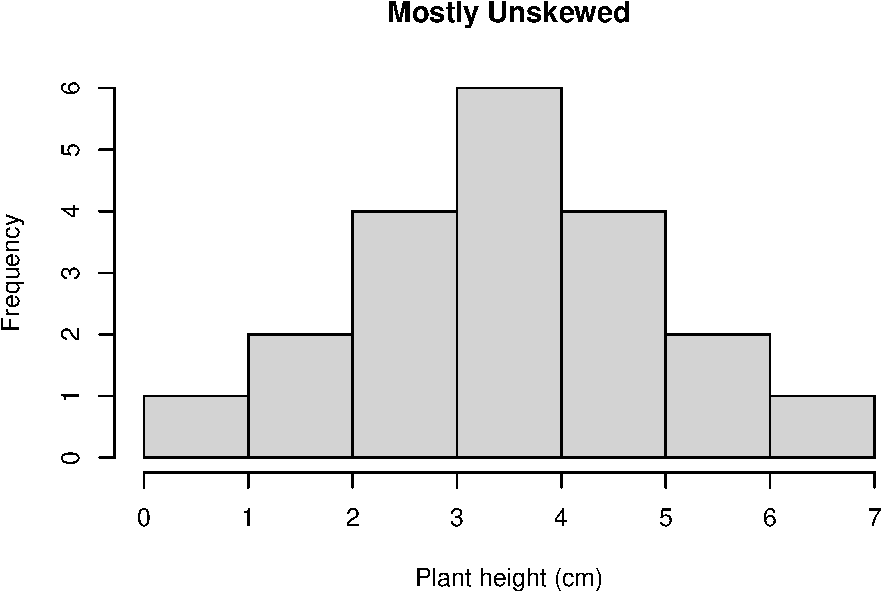
\includegraphics{_main_files/figure-latex/unnamed-chunk-10-1.pdf}
In this relatively unskewed example, the tails are approximately even. This shape is also referred to as a normal or Gaussian distribution.
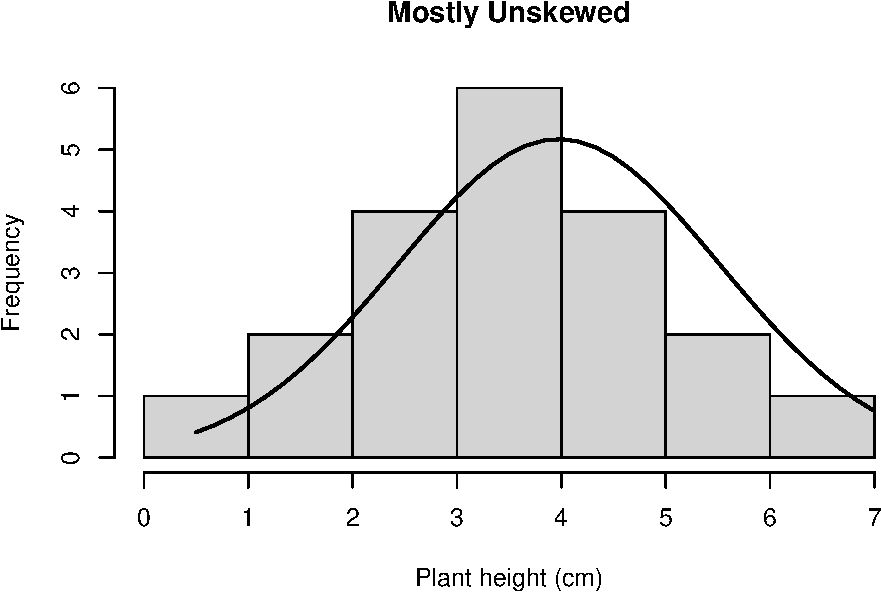
\includegraphics{_main_files/figure-latex/unnamed-chunk-11-1.pdf}
Here, we superimposed the bellshaped Normal or Gaussian distribution.

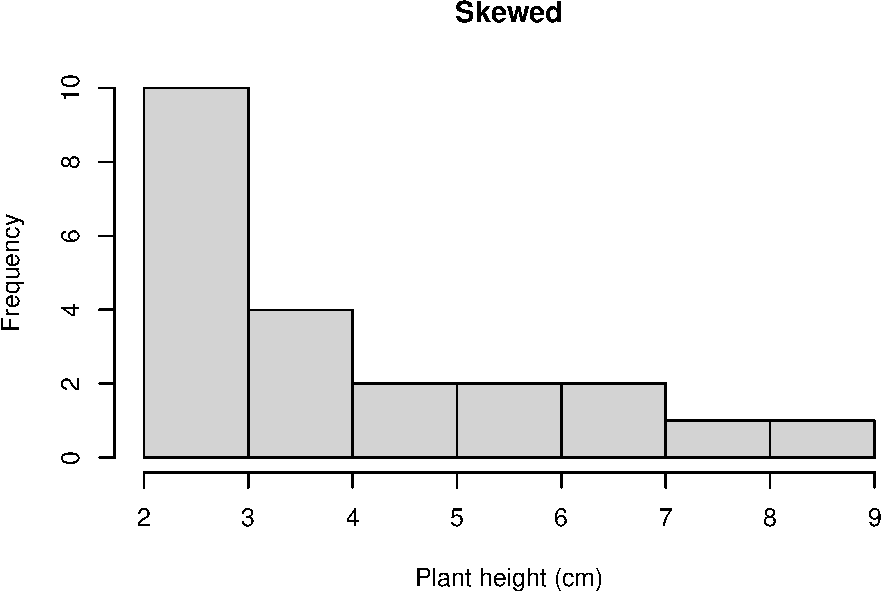
\includegraphics{_main_files/figure-latex/unnamed-chunk-12-1.pdf}
In this example of skewed data, the tail tapers to the right, indicated that the data is skewed to the right.

In order to explain outliers, we need to look at quantiles! Quantiles are proportions of your data, in other words a way to break your data into chunks to understand spread. You can break your data into as many quantiles as you would like, but it is most common to break your data into 4 parts, also called quartiles. (If you break data into 5 parts, the components are called quintiles, 10 parts = deciles, 100 parts = percentiles).

When you break data into quartiles, roughly 25 percent of the data occurs within each data chunk. The first chunk of the dataset contains 25\% of the data (25th percentile; 25\% of the data fall at or below this cut-off) is called the first quartile, the 50th percentile is called the sample median or the second quartile, the 75th percentile is called the third quartile.

Box and whisker plots are commonly used to quickly examine quartiles. Let's check out our plant height data again, using a box and whisker plot.
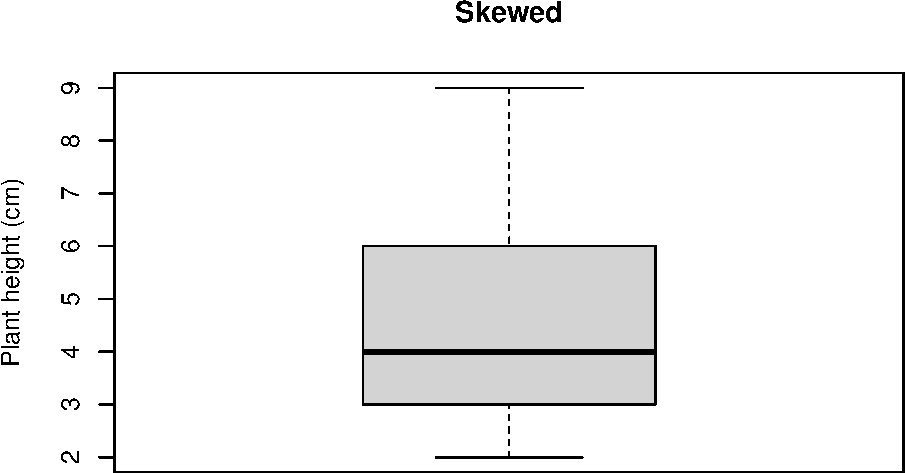
\includegraphics{_main_files/figure-latex/unnamed-chunk-13-1.pdf}
In the plot shown here, the box encapsulates the Interquartile Range (IQR); the center of the data ranging from the 25th percentile to the 75th. The black line in the middle of the box is the median (also called the 50th percentile, because it bisects the dataset; half of the data occur above the median and half below). The lines emerging from the box (whiskers) indicate the extent of the first and third quartiles, and usually corresponding with the minimum and maximum values of the dataset, unless there are \textbf{outliers}. An outlier is a datapoint that occurs outside of the 1st or 3rd quantile. Let's add one to our Sedona dataset, and see how it is represented on the box and whisker plot.

\begin{Shaded}
\begin{Highlighting}[]
\CommentTok{\#Let\textquotesingle{}s add a plant height of 20.}
\NormalTok{sedona\_skewed }\OtherTok{\textless{}{-}} \FunctionTok{c}\NormalTok{(}\DecValTok{3}\NormalTok{, }\DecValTok{3}\NormalTok{, }\DecValTok{3}\NormalTok{, }\DecValTok{3}\NormalTok{, }\DecValTok{7}\NormalTok{, }\DecValTok{3}\NormalTok{, }\DecValTok{4}\NormalTok{, }\DecValTok{5}\NormalTok{, }\DecValTok{6}\NormalTok{, }\DecValTok{3}\NormalTok{, }\DecValTok{3}\NormalTok{, }\DecValTok{3}\NormalTok{, }\DecValTok{4}\NormalTok{, }\DecValTok{4}\NormalTok{, }\DecValTok{6}\NormalTok{, }\DecValTok{7}\NormalTok{, }\DecValTok{8}\NormalTok{, }\DecValTok{9}\NormalTok{, }\DecValTok{3}\NormalTok{, }\DecValTok{4}\NormalTok{, }\DecValTok{5}\NormalTok{, }\DecValTok{2}\NormalTok{, }\DecValTok{20}\NormalTok{)}
\FunctionTok{boxplot}\NormalTok{(sedona\_skewed, }\AttributeTok{main=}\StringTok{"Skewed"}\NormalTok{, }\AttributeTok{ylab=}\StringTok{"Plant height (cm)"}\NormalTok{)}
\end{Highlighting}
\end{Shaded}

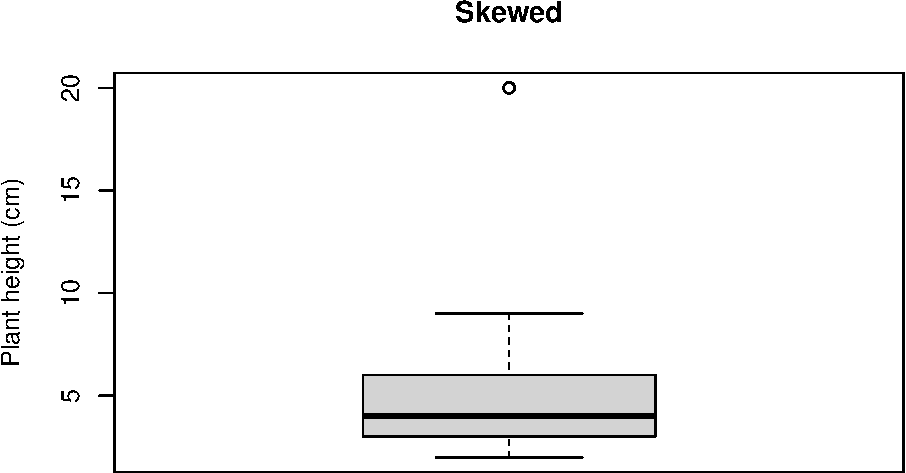
\includegraphics{_main_files/figure-latex/unnamed-chunk-14-1.pdf}
The outlier appears as a dot on the box and whisker plot, and is the maximum value of the dataset.

One other thing to note: Standard deviation also breaks data into meaningful segments, but is only used when data conform to a normal distribution; the mean +/- 1 SD accounts for 68\% of the data, +/-2 SDs contains 95\% of data, and +/- 3SD includes 99\% of data. That said, I've never presented standard deviation in a manuscript; it is much more common to include standard error or confidence intervals (discussed later).

We've played around a lot with data, but what do you actually need to take away from this?
\emph{Data types (Categorical, Numerical discrete, Numerical continuous, Ordinal)
\textbf{Why?} We will select analyses based on data type.
}The two basic questions that most statistical analyses answer.
\textbf{Why?} This will help you define what statistics can and can't do and bound our learning space!
\emph{Ways to describe numerical continuous data (Location, Spread, Shape, Outliers).
\textbf{Why?} You will describe your results using these concepts in write-up AND these concepts will be important for certain analyses.
}Know how to calculate mean, median, and standard error.
\textbf{Why?} These are typical ways to describe data in results sections.
\emph{Start to familiarize yourself with mathematical annotation.
\textbf{Why?} You may need to include equations in your methods section.
}Start to familiarize yourself with R code.
\textbf{Why?} Most researchers now use R to analyze, describe, and visualize their data.
*Be able to interpret a histogram and box-whisker plot.
\textbf{Why?} These are commonly used ways to visualize data.

Now, let's play around a little more with R! For your reference, here is a guide that shows the basics formulas for calculations in R: \href{downloads/calculator.pdf}{Supplementary Material}

Let's also try describing the petal lengths of 3 different plant species: Milkweed, Bluestar and Pectis using this dataset:
\href{downloads/lesson2data.csv}{Download the example dataset}
The code can be used to import the data, but in case you wanted to access the data yourself - provided above!

Build on this code, to generate your description of the petal lengths of your focal species:
\href{downloads/lesson2summarystatistics.R}{R Script for Chapter 1}

Please put your results in a document and submit to your TA in canvas!

  \bibliography{book.bib,packages.bib}

\end{document}
